\section{Paso de mensajes}

Cuando varios procesos cooperan entre sí deben satisfacer dos requisitos fundamentales:
\begin{itemize}
  \item \textit{Sincronización}: coordinar la ejecución de los procesos y garantizar la exclusión mutua cuando sea necesario.
  \item \textit{Comunicación}: intercambiar información entre procesos.
\end{itemize}

Una forma de satisfacer ambos requisitos es mediante el \textit{paso de mensajes} (\textit{message passing}), donde los procesos se comunican enviando y recibiendo mensajes, sin necesidad de compartir memoria.

Las primitivas fundamentales son:
\begin{ccode}
send(destination, message);
receive(source, message);
\end{ccode}

La operación \texttt{send()} envía un mensaje a un proceso destino, mientras que \texttt{receive()} recibe un mensaje proveniente de un proceso origen.

Los principales aspectos de diseño de un sistema de paso de mensajes se resumen en la Cuadro~\ref{tab:message-passing}.

\begin{table}[!ht]
\centering
\begin{tabular}{p{3.5cm}p{8.5cm}}
\toprule
\textit{Aspecto} & \textit{Opciones} \\
\midrule
Sincronización &
Envío: bloqueante o no bloqueante.\\
&
Recepción: bloqueante, no bloqueante o prueba de llegada del mensaje.\\
\addlinespace

Direccionamiento &
Directo (explícito o implícito).\\
&
Indirecto (estático, dinámico o por propiedad del buzón).\\
\addlinespace

Formato &
Contenido del mensaje.\\
&
Longitud fija o variable.\\
\addlinespace

Disciplina de colas &
FIFO o por prioridad.\\
\bottomrule
\end{tabular}
\caption{Aspectos de diseño de un sistema de paso de mensajes.}
\label{tab:message-passing}
\end{table}

\subsection{Sincronización}

El intercambio de mensajes implica un cierto grado de sincronización entre procesos, ya que un mensaje no puede recibirse antes de haber sido enviado. Por ello, un sistema de paso de mensajes debe definir qué ocurre con un proceso después de ejecutar las primitivas \texttt{send()} y \texttt{receive()}.

Tanto el envío como la recepción pueden ser \textit{bloqueantes} o \textit{no bloqueantes}:

\begin{itemize}
  \item \textit{Envío bloqueante}: el proceso emisor permanece bloqueado hasta que el mensaje es recibido.
  \item \textit{Envío no bloqueante}: el proceso continúa su ejecución inmediatamente después de enviar el mensaje.
  \item \textit{Recepción bloqueante}: si el mensaje aún no está disponible, el proceso receptor queda bloqueado hasta recibirlo.
  \item \textit{Recepción no bloqueante}: si no existe un mensaje disponible, el proceso continúa su ejecución sin esperar.
\end{itemize}

Las combinaciones más utilizadas se muestran en el Cuadro \ref{tab:combinaciones_de_sincronizacion}.

\begin{table}[!ht]
\centering
\begin{tabular}{>{\footnotesize\raggedright\arraybackslash}p{3.7cm} >{\footnotesize}p{9cm}}
\toprule
\normalsize\textit{Combinación} & \normalsize\textit{Características} \\
\midrule
Envío y Recepción bloqueantes &
Ambos procesos esperan hasta que el mensaje es entregado (\textit{rendezvous}), proporcionando una sincronización estricta. \\
\addlinespace

Envío no bloqueante y Recepción bloqueante &
El emisor continúa inmediatamente, mientras que el receptor espera hasta recibir el mensaje. Es la combinación más utilizada, especialmente en arquitecturas cliente-servidor. \\
\addlinespace

Envío y Recepción no bloqueante &
Ninguno de los procesos espera al otro. Proporciona mayor paralelismo, pero requiere mecanismos adicionales para comprobar la llegada de mensajes. \\
\bottomrule
\end{tabular}
\caption{Combinaciones de sincronización en el paso de mensajes.}
\label{tab:combinaciones_de_sincronizacion}
\end{table}

El envío no bloqueante permite que un proceso continúe realizando otras tareas sin esperar la recepción del mensaje, aunque normalmente requiere algún mecanismo de confirmación para garantizar que el mensaje fue recibido.

Por su parte, la recepción bloqueante suele ser la opción más natural, ya que un proceso normalmente necesita el mensaje antes de continuar. Sin embargo, en sistemas distribuidos puede provocar esperas indefinidas si el mensaje nunca llega. En estos casos pueden emplearse recepciones no bloqueantes o primitivas que permitan comprobar la llegada de un mensaje antes de intentar recibirlo.

\subsection{Direccionamiento}

El paso de mensajes requiere un mecanismo para identificar el origen y el destino de cada mensaje. Existen dos enfoques principales: \textit{direccionamiento directo} e \textit{indirecto}.

\subsubsection{Direccionamiento directo}

En el direccionamiento directo, el proceso emisor especifica explícitamente el proceso destino en la operación \texttt{send()}. La recepción puede realizarse de dos formas:
\begin{itemize}
  \item \textit{Explícita}: el receptor indica de qué proceso espera recibir el mensaje.
  \item \textit{Implícita}: el receptor acepta un mensaje de cualquier proceso y la operación \texttt{receive()} devuelve la identidad del emisor.
\end{itemize}

El direccionamiento explícito es adecuado cuando los procesos conocen previamente con quién deben comunicarse, mientras que el implícito resulta útil para procesos que atienden solicitudes provenientes de múltiples orígenes.

\subsubsection{Direccionamiento indirecto}

En el direccionamiento indirecto, los procesos no intercambian mensajes directamente, sino a través de un \textit{buzón} (\textit{mailbox}) o \textit{puerto} (\textit{port}), que actúa como una cola temporal de mensajes.

Este mecanismo desacopla al emisor y al receptor, permitiendo distintas formas de comunicación:
\begin{itemize}
  \item Uno a uno.
  \item Muchos a uno (cliente-servidor).
  \item Uno a muchos (difusión).
  \item Muchos a muchos.
\end{itemize}

La asociación entre procesos y buzones puede ser:
\begin{itemize}
  \item \textit{Estática}: el buzón se asigna permanentemente al proceso.
  \item \textit{Dinámica}: la asociación se establece y elimina durante la ejecución mediante operaciones como \texttt{connect()} y \texttt{disconnect()}.
\end{itemize}

Finalmente, los buzones pueden pertenecer al proceso que los crea o al propio sistema operativo. En el primer caso, el buzón desaparece al finalizar el proceso; en el segundo, permanece hasta que sea eliminado explícitamente.

\subsection{Formato de los mensajes}

El formato de un mensaje depende del sistema de paso de mensajes. Existen dos enfoques principales:
\begin{itemize}
  \item \textit{Longitud fija}: reduce el costo de procesamiento y almacenamiento, aunque limita la cantidad de información que puede enviarse.
  \item \textit{Longitud variable}: ofrece mayor flexibilidad, siendo el formato más utilizado.
\end{itemize}
En general, un mensaje de longitud variable se divide en dos partes:
\begin{itemize}
  \item \textit{Cabecera}: contiene información de control, como origen, destino, longitud, tipo de mensaje, prioridad o número de secuencia.
  \item \textit{Cuerpo}: contiene los datos que se desean transmitir.
\end{itemize}

\begin{figure}[!ht]
  \centering
  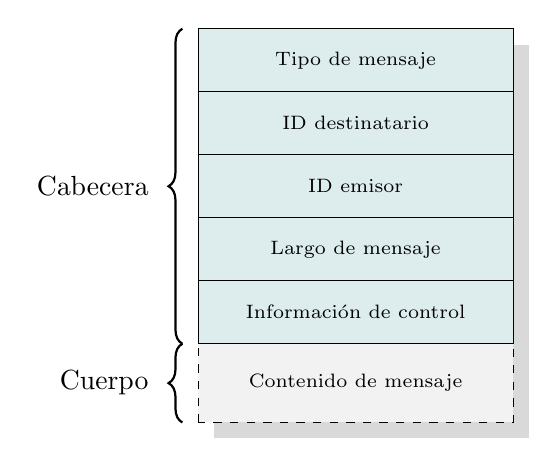
\begin{tikzpicture}
    \fill[gray!30] (.2,-.2) rectangle (4.2,4.8);
    % body
    \draw[dashed,fill=gray!10] (0,0) rectangle node[font=\scriptsize]{Contenido de mensaje} (4,1);
    % header
    \draw[fill=white!93!green!93!blue] (0,1) rectangle node[font=\scriptsize]{Información de control} (4,1.8);
    \draw[fill=white!93!green!93!blue] (0,1.8) rectangle node[font=\scriptsize]{Largo de mensaje} (4,2.6);
    \draw[fill=white!93!green!93!blue] (0,2.6) rectangle node[font=\scriptsize]{ID emisor} (4,3.4);
    \draw[fill=white!93!green!93!blue] (0,3.4) rectangle node[font=\scriptsize]{ID destinatario} (4,4.2);
    \draw[fill=white!93!green!93!blue] (0,4.2) rectangle node[font=\scriptsize]{Tipo de mensaje} (4,5);
    
    % body bracket     
    \draw [decorate, decoration={brace, amplitude=5pt}, thick] 
          (-.2, 0) -- (-.2, 1) node [midway, left=0.3cm] {Cuerpo};
    % header bracket
    \draw [decorate, decoration={brace, amplitude=5pt}, thick] 
          (-.2, 1) -- (-.2, 5) node [midway, left=0.3cm] {Cabecera};
  \end{tikzpicture}
  \caption{Formato general de mensaje.}
\end{figure}

\subsection{Disciplina de colas}

Los mensajes almacenados en un buzón pueden ordenarse siguiendo distintas políticas:
\begin{itemize}
  \item \textit{FIFO}: los mensajes se reciben en el mismo orden en que fueron enviados.
  \item \textit{Prioridad}: los mensajes más importantes se entregan antes que el resto.
\end{itemize}
En algunos sistemas también se permite que el proceso receptor inspeccione la cola y seleccione qué mensaje recibir.

\subsection{Exclusión mutua}

La exclusión mutua puede implementarse mediante un buzón compartido que inicialmente contiene un único mensaje. Dicho mensaje actúa como un \textit{testigo} (\textit{token}): únicamente el proceso que logra recibirlo puede acceder a la sección crítica. Al finalizar, devuelve el mensaje al buzón para que otro proceso pueda continuar.

\begin{ccode}[title=Programa de exclusión mutua usando paso de mensajes]
const int n = /* número de procesos */;

void P(int i) {
  message msg;
  while (true) {
    receive(box, msg); // bloqueante
    /* sección crítica */
    send(box, msg); // no bloqueante
    /* remainder */
  }
}

void main() {
  create_mailbox(box);
  send(box, null); // no bloqueante
  parbegin(P(1), P(2), ..., P(n));
}
\end{ccode}

Este mecanismo supone que cada mensaje es entregado a un único proceso y que, si el buzón está vacío, los procesos que intenten recibir un mensaje permanecerán bloqueados.

\subsection{Productor-consumidor}

El problema productor--consumidor puede resolverse utilizando dos buzones:
\begin{itemize}
  \item \texttt{mayproduce}: controla la cantidad de posiciones libres del búfer.
  \item \texttt{mayconsume}: almacena los elementos producidos.
\end{itemize}

Inicialmente, \texttt{mayproduce} contiene tantos mensajes vacíos como capacidad tenga el búfer. Cada productor consume uno de esos mensajes antes de producir un elemento y lo reemplaza por un mensaje con datos en \texttt{mayconsume}. El consumidor realiza la operación inversa: recibe un elemento de \texttt{mayconsume}, lo procesa y devuelve un mensaje vacío a \texttt{mayproduce}.

\begin{ccode}[title=Problema productor-consumidor con paso de mensajes]
const int capacity = /* capacidad del buffer */;
null = /* mensaje vacío */;

void producer() {
  message pmsg;
  while (true) {
    receive(mayproduce, pmsg); // bloqueante
    pmsg = produce();
    send(mayconsume, pmsg); // no bloqueante
  }
}

void consumer() {
  message cmsg;
  while (true) {
    receive(mayconsume, cmsg); // bloqueante
    consume(cmsg);
    send(mayproduce, null); // no bloqueante
  }
}

void main() {
  create_mailbox(mayproduce);
  create_mailbox(mayconsume);
  for (int i = 1; i <= capacity; i++)
    send(mayproduce, null); // no bloqueante
  parbegin(producer, consumer);
}
\end{ccode}

Esta solución admite múltiples productores y consumidores, e incluso puede utilizarse en sistemas distribuidos, ya que toda la coordinación se realiza mediante el intercambio de mensajes.
